% \iffalse meta comment
% File: adfathesis.dtx
%
%   ADFATHESIS.CLS by Stephen Harker, Dept. of Physics, ADFA: 12-JUN-94
%   These macros are placed in the public domain.  They may be freely
%   transmitted, reproduced, or modified.  No rights are reserved.
%
%   This is based on the Monash University version of SUTHESIS.STY called
%   MONTHESIS.STY by Tony McGrath, Dept. of Physics, Monash Uni: 5-NOV-87
%   and the ADFATHESIS.STY that is/was on ccadfa.cc.adfa.oz.au
%
%   PhD thesis style --- modifications to the REPORT class:
%   Style information from the `1993 Handbook' for the University College
%   known as the `Blue Book', see pages 168 to 170.  Updated for 1997. 
%
%   This program is distributed in the hope that it will be useful,
%   but WITHOUT ANY WARRANTY; without even the implied warranty of
%   MERCHANTABILITY or FITNESS FOR A PARTICULAR PURPOSE.
%
% \fi
% \CheckSum{1075}
%% \CharacterTable
%%  {Upper-case    \A\B\C\D\E\F\G\H\I\J\K\L\M\N\O\P\Q\R\S\T\U\V\W\X\Y\Z
%%   Lower-case    \a\b\c\d\e\f\g\h\i\j\k\l\m\n\o\p\q\r\s\t\u\v\w\x\y\z
%%   Digits        \0\1\2\3\4\5\6\7\8\9
%%   Exclamation   \!     Double quote  \"     Hash (number) \#
%%   Dollar        \$     Percent       \%     Ampersand     \&
%%   Acute accent  \'     Left paren    \(     Right paren   \)
%%   Asterisk      \*     Plus          \+     Comma         \,
%%   Minus         \-     Point         \.     Solidus       \/
%%   Colon         \:     Semicolon     \;     Less than     \<
%%   Equals        \=     Greater than  \>     Question mark \?
%%   Commercial at \@     Left bracket  \[     Backslash     \\
%%   Right bracket \]     Circumflex    \^     Underscore    \_
%%   Grave accent  \`     Left brace    \{     Vertical bar  \|
%%   Right brace   \}     Tilde         \~}
%
% \iffalse
%<package>\NeedsTeXFormat{LaTeX2e}
%<package>\ProvidesClass{adfathesis}
%<package>         [2004/04/16 \space v2.50 \space ADFA thesis class]
%
%<*driver>
\documentclass{ltxdoc}
 \title{The \texttt{adfathesis} class}
 \author{Stephen Harker}
 \date{Printed \today}
 \MakeShortVerb{\=}
 \MakeShortVerb{\"}
 \newcommand{\bs}{\char '134 }  % A backslash character for \tt font
\begin{document}
 \maketitle
 \DeleteShortVerb{\|}
 \DocInput{adfathesis.dtx}
\end{document}
%</driver>
% \fi
%
% \begin{abstract}
% This article describes the \textsf{adfathesis} class, which is designed as
% the ADFA
% PhD thesis style --- a modification to the \textsf{report} class:
% Style information from the `1993 Handbook' for the University College
% known as the `Blue Book', see pages 168 to 170.  Updated for 1997. 
% This version is modified only to use the \textsf{docstrip} mechanism.
% \end{abstract}
%
% \section{Introduction}
%
% The adfathesis class is based on the Monash University version of
% \textsf{suthesis.sty}  called
% \textsf{monthesis.sty} by Tony McGrath, Dept. of Physics, Monash Uni: 5-NOV-87
% and the \textsf{adfathesis.sty} that is/was on ccadfa.cc.adfa.oz.au.  
%
% Some basic information on
% the use of \textsf{adfathesis} follows.  This class file can only be used
% under \LaTeXe.  Firstly an example of use:

% \begin{quote}
% \small
% \begin{verbatim}
% \documentclass[a4paper,12pt,openright,twoside]{adfathesis}

% % Control which chapters are LaTeX'd in this run with

% \includeonly{chapter1,chapter2,chapter3}

% \title{How to Write Theses\\
%        With Two Line Titles}
% \authornameonly{John Henry Candidate}
% \author{\Authornameonly \\ B.Sc.(Hons)}
% \copyrightfalse     % No copyright page
% \figurespagefalse   % No List of Figures
% \tablespagefalse    % No List of Tables

% \begin{document}
% \beforepreface
% \prefacesection{Abstract}
%     This thesis tells you all you need to know about...
% \declaration   % Declaration page
% \prefacesection{Acknowledgements}
%     I would like to thank...
% \afterpreface
 
% % Sample University of Calgary Thesis
% This file contains CHAPTER ONE

\chapter{Introduction}

\epigraph{Lorem ipsum dolor sit amet,
consectetuer adipiscing elit.}{Anonymous}

The text above is an \emph{epigraph}. In this typeface, you can have
text in \textbf{boldface}, \emph{italics}, \textbf{\emph{bold
    italics}}, \textsl{slanted}, and \textsc{Small Caps}.

\section{Literature Review}

\blindtext\pagenote{\blindtext}

\blindtext[2]

\begin{defn}
A group~$G$ is said to be \emph{abelian} (or \emph{commutative}) if
for every $a, b \in G$, $a \cdot b = b \cdot a$.
\end{defn}

\blindtext[2]

\section{Contributions of the Thesis}

\blindtext[3]

\begin{table}
  \begin{center}
  \begin{tabular}{c|c}
    A & B \\
    \hline
    1 & 2
  \end{tabular}
  \end{center}
  \caption{Letters and numbers}
\end{table}

\blindtext[3]
  % Introduction
%          ...
% \include{chapter6}  % Conclusions
%          ...
% \appendix
% \chapter{Test Appendix with a very long title in order to test spacing behavior} \label{app:test}
\lipsum[2]

A convenient form for representing substantial numerical or textual data is a table. 
Table~\ref{tab:test} shows an example of this functionality in \LaTeX.
\begin{table}
  \centering
  \caption{Test table. With an extra-long caption to test spacing functionality for table captions. And inline mathematics.}
  \begin{tabular}{lrr}
    \toprule
    Heading 1 ($u_x$)  & Head 2 & Head 3 \\
    \midrule
    Analytical         & 1.000  & 1.000  \\
    Forward Difference & 0.973  & 0.976  \\
    \bottomrule
  \end{tabular}
  \label{tab:test}
\end{table}
Diagrams, plots, and other graphics should be placed in figures. 
Figure~\ref{fig:test} shows an example of such an environment.
The command \verb+\includegraphics+ from the \verb+graphicx+ package may be used to include external graphics in a wide variety of formats.
\begin{figure}
  \centering 
  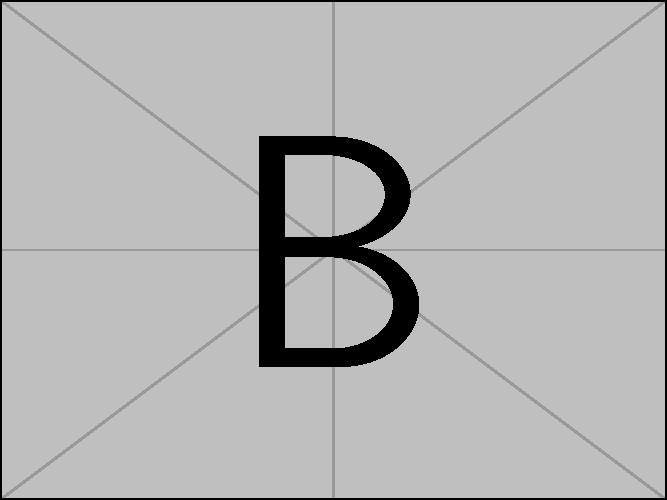
\includegraphics[width=1in]{example-image-b}
  \caption{This test figure tests captions and Table of Contents 
    behavior for lengthy captions.}
  \label{fig:test}
\end{figure}

\section{This is a Very Long Heading to Test the Table of Contents Behavior for Very Long Section Headings}
Sample text. Sample text.

\subsection{This is an Extremely Long Subsection Heading to Test Spacing Behavior for Subsections}
\lipsum[3]

\subsubsection{This is an Extremely Long Subsubsection Heading to Test Spacing Behavior for Subsubsections}
\lipsum[4-5]
 % A Long Proof
%          ...
% \clearpage                                        % Needed to get page 
% \addcontentsline{toc}{chapter}{References}        % in TOC correct. 
% \bibliographystyle{adfathesis}
% \bibliography{mybib}
% \end{document}
% \end{verbatim}
% \end{quote}

% \section{Documentation:} 
% This class modifies the standard report class
% to meet the \textsc{adfa} requirements given in the `\emph{University
%   College Handbook}'.  It sets the margins, interline spacing, the
% figure and table numbering style, and disallows page breaks at
% hyphens.

% The `\texttt{\bs{}beforepreface}' command creates the title page, a
% copyright page (optionally), and the table of contents.  Then the user
% should put preface section(s), using the command
% `\texttt{\bs{}prefacesection\{}\emph{Section Title}\texttt{\}}', this
% should include the declaration page.  The tables of tables and figures
% are then produced by the `\texttt{\bs{}afterpreface}' command, which
% also sets things up to start the main body (on arabic page~1).

% The following commands can control what goes in the front matter
% material:
% \begin{description}
% \small
% \item{\ttfamily\bs{}title\{\emph{thesis title}\}} Title of the thesis.
% \item{\ttfamily\bs{}authornameonly\{\emph{name}\}} The author's name
%   without degrees earned, needed for the declaration.
% \item{\ttfamily\bs{}author\{\emph{name}\}} The author's name with
%   degrees earned, for the titlepage.
% \item{\ttfamily\bs{}dept\{\emph{department}\}} The default value is
%   School of `\emph{Physics}'.
% \item{\ttfamily\bs{}thesistype\{\emph{Type of thesis}\}} The default
%   value is `\emph{Doctor of Philosophy}', for an Honours report this should
%   be the faculty (e.g.\ `\emph{Science}').
% \item{\ttfamily\bs{}degreetype\{\emph{Faculty for degree}\}} The default
%   value is `\emph{Science}', used for Honours only.
% \item{\ttfamily\bs{}submitdate\{\emph{date}\}} Month and year in which
%   submitted; date \LaTeX{}'d if omitted.
% \item{\ttfamily\bs{}copyrightyear\{\emph{year}\}} Year degree
%   conferred, or year \LaTeX{}'d if omitted (next year if in December).
% \item{\ttfamily\bs{}declaration} Produce the required declaration that
%   the thesis is all the author's own work.
% \item{\ttfamily\bs{}copyrighttrue} Produce or
%   \texttt{\bs{}copyrightfalse} don't produce a `\emph{copyright}' page
%   (true by default).
% \item{\ttfamily\bs{}figurespagetrue} Produce or
%   \texttt{\bs{}figurespagefalse} don't produce a `\emph{List of
%     Figures}' page (true by default).
% \item{\ttfamily\bs{}tablespagetrue} Produce or
%   \texttt{\bs{}tablespagefalse} don't produce a `\emph{List of
%     Tables}' page (true by default).
% \end{description}

% This class uses space and a half interline spacing, except in
% footnote, figure and table environments where normal spacing is used.
% The command: `\texttt{\bs{}linespread\}\-\{1.655\}}' can be used to
% change this (use whatever you want instead of 1.655).  For 12 point
% Computer Modern fonts 1.241 corresponds to space and a half, and 1.655
% to double spacing.  This command should be given in the preamble
% (i.e.\ before the `\texttt{\bs{}begin\{document\}}').

% The example given shows the \textsf{12pt} option being used.  This is
% required by the 1997 handbook, but may be omitted (at your own risk)
% to get smaller print.  There are three options which may be declared
% in \texttt{\bs{}documentclass[a4paper,12pt]\{adfathesis\}}:
% \begin{itemize}
% \item \texttt{draft} which changes the pagestyle to include the date
%   on the page header.
% \item \texttt{normalbib} which stops the document using the
%   \textsf{Harvard} style, and hence allows use of either the standard
%   \LaTeX\ bibliography style or an alternative package.  The supplied
%   \textsf{adfathesis.bst} may not be appropriate in this case. so you
%   could use an alternative such as \textsf{plain.bst}.
% \item \textsf{honours} which changes the titlepage to one more
%   appropriate to an Honours report.  
% \end{itemize}

% To get the correct page number for the bibliography in the table of
% contents you need to put a `\texttt{\bs{}clearpage}' command before
% the `\texttt{\bs{}addcontentsline}' command.  The thickness of the
% rules used for the chapter headings is controlled by
% `\texttt{\bs{}chaprule}' and can be set to another value, say 0~pt, by
% the command `\texttt{\bs{}setlength\{\bs{}chaprule\}\{0pt\}}' in the
% preamble. There is a maximum value of 6~pt for
% `\texttt{\bs{}chaprule}'.
%
% \StopEventually
%
% \section{The code\label{code}}
%    The current version is defined at the top of the file looking
%    something like this
%    \begin{macrocode}
%<*package>
%\NeedsTeXFormat{LaTeX2e}
%\ProvidesPackage{adfathesis}
%        [\filedate\space version\fileversion]
%    \end{macrocode}
%
% First we set up some new flags:
% A new flag for draft printing,
% at this stage all I do is reset the page style.  
% This is not true by default, must be changed in the thesis BASE file
% A new flag whether to use the Harvard bib package?
% This is true by default, must be changed  in the thesis BASE file
% A new flage whether a Honours report rather than PhD or Masters thesis?
% This is not true by default, must be changed in the thesis BASE file
%    \begin{macrocode}
\newif\ifATdr@ft         
\ATdr@ftfalse            
\newif\ifAT@harvbib      
\AT@harvbibtrue          
\newif\ifATh@nours       
\ATh@noursfalse          
%    \end{macrocode}
%
% Now we define the default values for the flags, and
% make 12 point text the default.
%
%    \begin{macrocode}
\newcommand{\ptsize}{}
\DeclareOption{draft}
   {\ATdr@fttrue
    \PassOptionsToClass{draft}{report}}
\DeclareOption{normalbib}
   {\AT@harvbibfalse}
\DeclareOption{harvard}
   {\AT@harvbibtrue}
\DeclareOption{honours}
   {\ATh@nourstrue}
\DeclareOption{10pt}{\renewcommand{\ptsize}{10pt}}
\DeclareOption{11pt}{\renewcommand{\ptsize}{11pt}}
\DeclareOption{12pt}{\renewcommand{\ptsize}{12pt}}
\DeclareOption*{\PassOptionsToClass{\CurrentOption}{report}}
\ExecuteOptions{12pt}
%    \end{macrocode}
% Now process the options and load the standard report class.  We merely
% make modifications to the report classs.
%
%    \begin{macrocode}
\ProcessOptions\relax
\LoadClass[a4paper,\ptsize]{report}
\ifAT@harvbib\IfFileExists{harvard.sty}{\RequirePackage{harvard}}%
  {\ClassError{\filename}{%
  The Harvard package was not found.}{%
  The Harvard package controls the bibliography appearance. \MessageBreak
  \space It is used by default unless you specify the normalbib option. \MessageBreak
  \space The Harvard package can be obtained from, e.g., ctan.unsw.edu.au
  }}\fi
%    \end{macrocode}
% From the Blue book we find the following regulations:
% The size of the paper shall approximate A4 (297mm x 210 mm).
% The margins on each sheet shall be not less than 40mm on the left
% hand side, 20mm on the right hand side, 30mm at the top and 20mm at
% the bottom.
% \TeX\ has default margins of 1 inch (25.4mm) at the top and left.
%
% Use the code from \textsf{size12.clo} to set \verb|\textheight| to an integer
% multiple of \verb|\baselineskip|s.  Use \verb|\raggedbottom| and add one
% \verb|\baselineskip| to \verb|\topskip| to allow pagelength to vary.
%    \begin{macrocode}
\setlength{\oddsidemargin}  {1.5cm}
\setlength{\evensidemargin} {-0.5cm}    
\setlength{\marginparwidth} {40\p@}
\setlength{\marginparsep}   {10\p@}     
\setlength{\topmargin}      {-0.6cm}    
\setlength{\headheight}     {15\p@}     
\setlength{\headsep}        {0.5cm}
\setlength{\textwidth}      {14.9cm}    
\setlength\@tempdima{\paperheight}
\addtolength\@tempdima{-30mm}  
\addtolength\@tempdima{-20mm}  
\divide\@tempdima\baselineskip
\@tempcnta=\@tempdima
\setlength\textheight{\@tempcnta\baselineskip}
\addtolength\textheight{\topskip}
\setlength{\topskip}{1\topskip \@plus 1\baselineskip}
\setlength{\parskip}{0pt}
\raggedbottom
%    \end{macrocode}
%
% Set spacing for space and a half, using values from setspace.sty.
% Use the new \verb|\linespread| command rather than 
% \verb|\renewcommand{\baselinestretch}{1.25}| etc.
%    \begin{macrocode}
\ifcase \@ptsize \relax % 10pt
  \linespread{1.25}%
\or % 11pt
  \linespread{1.213}%
\or % 12pt
  \linespread{1.241}%
\fi
%    \end{macrocode}
%
% Next two sections taken from \textsf{setspace}.
%    \begin{macrocode}
\newcommand{\displayskipstretch}{\baselinestretch}
\newcommand{\setdisplayskipstretch}[1]{\renewcommand{\displayskipstretch}{#1}}
%    \end{macrocode}
%
% Fix up spacing before and after displayed math
% (\verb|arraystretch| seems to do a fine job for inside LaTeX
% displayed math, 
% since \verb|array| and \verb|eqnarray| seem to be affected as expected).
% Changing \verb|\baselinestretch| and doing a font change also works
% if done here, 
% but then you have to change \verb|@setsize| to remove the call to
% \verb|@nomath|).
%
%    \begin{macrocode}
\everydisplay\expandafter{%
  \the\everydisplay
  \abovedisplayskip \displayskipstretch\abovedisplayskip
  \belowdisplayskip \displayskipstretch\belowdisplayskip
  \abovedisplayshortskip \displayskipstretch\abovedisplayshortskip
  \belowdisplayshortskip \displayskipstretch\belowdisplayshortskip
}
%    \end{macrocode}
%
% The Following changed by Stephen Harker, October 1993 to:%
%  \begin{itemize}
%  \item   Make Chapter title centred, and modify size to \verb|\Large| not
%        \verb|\Huge|, use small caps for `chapter' and rules above and 
%        below.  Rule thickness defined by new length \verb|\chaprule|.
%        To change this use \verb|\setlength|.  
%       The value is forced to be less than 6 points below!
%  \item  Make corresponding reductions to size of section,
%        subsection and subsubsection headers.
%  \item Rename Bibliography section to References.
%  \end{itemize}
%    \begin{macrocode}
\newlength{\chaprule}    
\newlength{\ATchapskip}
\setlength{\chaprule}{0.4\p@}
\setlength{\ATchapskip}{10\p@}
\advance \ATchapskip by -1\chaprule
\renewcommand{\@makechapterhead}[1]{%
  \ifdim\chaprule>6\p@ \setlength{\chaprule}{6\p@}\fi
  \vspace*{\ATchapskip}%
  \noindent\rule{\textwidth}{\chaprule}\par%
  \vskip 10\p@
  {\parindent \z@ \centering \normalfont
    \ifnum \c@secnumdepth >\m@ne
        {\Large\scshape \@chapapp\space \thechapter}
        \par\nobreak
        \vskip 8\p@
    \fi
    \interlinepenalty\@M
    \Large #1\par\nobreak
    \vskip 10\p@
    \noindent\rule{\textwidth}{\chaprule}\par%
    \vskip\ATchapskip
  }}
\renewcommand{\@makeschapterhead}[1]{%
  \ifdim\chaprule>6\p@ \setlength{\chaprule}{6\p@}\fi
  \vspace*{\ATchapskip}%
  \noindent\rule{\textwidth}{\chaprule}\par%
  \vskip 10\p@
  {\parindent \z@ \centering
    \normalfont
    \interlinepenalty\@M
    \Large #1\par\nobreak
    \vskip 10\p@
    \noindent\rule{\textwidth}{\chaprule}\par%
    \vskip\ATchapskip
  }}

\renewcommand{\section}{\@startsection{section}{1}{\z@}%
    {-1.5ex \@plus-1ex \@minus -.2ex}{0.8ex \@plus.2ex}%
    {\normalfont\large\raggedright}}
\renewcommand{\subsection}{\@startsection{subsection}{2}{\z@}%
    {-1.2ex \@plus -.5ex \@minus-.2ex}{0.5ex \@plus.1ex}%
    {\normalfont\normalsize\itshape\raggedright}}
\renewcommand{\subsubsection}{\@startsection{subsubsection}{3}{\z@}%
    {-1.0ex\@plus -.5ex \@minus -.2ex}{0.3ex \@plus .1ex}%
    {\normalfont\normalsize\itshape\raggedright}}
\renewcommand{\paragraph}{\@startsection{paragraph}{4}{\z@}%
    {1.0ex \@plus.5ex \@minus.2ex}{-1em}%
    {\normalfont\normalsize\itshape\raggedright}}
\renewcommand{\subparagraph}{\@startsection{subparagraph}{5}{\parindent}%
    {1.0ex \@plus.5ex \@minus .2ex}{-1em}%
    {\normalfont\normalsize\itshape\raggedright}}

\renewcommand{\bibname}{References}
%    \end{macrocode}
%
% The following is taken from \textsf{sober.sty}, Nico Poppelier and
% \textsf{rapport1.cls} (NTG classes). 
% Makes list (\texttt{enumerate} and \texttt{itemize}) more reasonable
% in vertical space, 
% by adjusting the spacing between items.
% Unfortunately in the \verb|size*.clo| files \verb|\small| etc also
% redefine these 
% values.  We could redefine \verb|\small| etc, but they are size dependent!
% Leave alone, since \verb|\small| is not usually used as an environment, at
% least not for large sections of a document.
%    \begin{macrocode}
\def\@listi{\leftmargin\leftmargini
    \labelsep .5em%
    \labelwidth\leftmargini
    \advance\labelwidth-\labelsep
    \parsep \z@
    \topsep 0.4ex \@plus\p@ 
    \itemsep 0\p@ \@plus1\p@}
\let\@listI\@listi
\@listi
\def\@listii{\leftmargin\leftmarginii
    \labelsep .5em%
    \labelwidth\leftmarginii
    \advance\labelwidth-\labelsep
    \topsep 0\p@ \@plus\p@
    \parsep \z@ \@plus\p@
    \itemsep \parsep}
\def\@listiii{\leftmargin\leftmarginiii
    \labelsep .5em%
    \labelwidth\leftmarginiii
    \advance\labelwidth-\labelsep
    \topsep 0\p@ \@plus\p@
    \parsep \z@
    \partopsep \z@ \@plus\p@
    \itemsep \topsep}
\def\@listiv{\leftmargin\leftmarginiv
    \labelsep .5em%
    \labelwidth\leftmarginiv
    \advance\labelwidth-\labelsep
    \topsep 0\p@ \@plus\p@
    \parsep \z@
    \partopsep \z@ \@plus\p@
    \itemsep \topsep}
\def\@listv{\leftmargin\leftmarginv
     \labelsep  .5em%
     \labelwidth\leftmarginv
     \advance\labelwidth-\labelsep%
     \topsep    0\p@ \@plus\p@
     \parsep    \z@
     \itemsep   \z@ \@plus\p@}
\def\@listvi{\leftmargin\leftmarginvi
     \labelsep  .5em
     \labelwidth\leftmarginvi
     \advance\labelwidth{-\labelsep}%
     \topsep    0\p@ \@plus\p@
     \parsep    \z@
     \itemsep   \z@ \@plus\p@}
%    \end{macrocode}
%
% Next re-define \verb|\cleardoublepage| as recommended by Piet van
% Oostrum in the 
% documentation for \textsf{fancyhdr.sty} page 15.  This is to avoid
% blank pages having headers or footers.
%    \begin{macrocode}
\renewcommand{\cleardoublepage}{\clearpage\if@twoside \ifodd\c@page\else
   \thispagestyle{empty}
   \hbox{}\newpage\if@twocolumn\hbox{}\newpage\fi\fi\fi}
%    \end{macrocode}
%
%  Reduce widow/orphan problems, mainly from a posting from Donald
%  Arsenau on \texttt{comp.text.tex}, 24 Sep 1995.
%  Updated to follow comments from Michael Downes on \texttt{comp.text.tex},
%  31 Aug 1998.
%    \begin{macrocode}
\doublehyphendemerits=10000     % No consecutive line hyphens.
\brokenpenalty=4991             % Reduce broken words across columns/pages.
\widowpenalty=9999              % Almost no widows at bottom of page.
\clubpenalty=9996               % Almost no orphans at top of page.
\interfootnotelinepenalty=9999  % Almost never break footnotes.
\predisplaypenalty=10000        % Default value
\postdisplaypenalty=1549        % Few breaks between display and widows
\displaywidowpenalty=1602       % At least as high as \postdisplaypenalty
%    \end{macrocode}
%
% Change float placement parameters to reduce problems.  Based on
% values posted by Donald Arsenau on \texttt{comp.text.tex} at various times.
% See in particular 17th Nov 1997.
%    \begin{macrocode}
\renewcommand{\topfraction}{.85}
\renewcommand{\bottomfraction}{.7}
\renewcommand{\textfraction}{.15}
\renewcommand{\floatpagefraction}{.66}
\renewcommand{\dbltopfraction}{.66}
\renewcommand{\dblfloatpagefraction}{.66}
\setcounter{topnumber}{9}
\setcounter{bottomnumber}{9}
\setcounter{totalnumber}{20}
\setcounter{dbltopnumber}{9}
%    \end{macrocode}
%
%  Make tables and figures default to small text and be single spaced,
%  and modify caption macro to allow this to take effect in the caption.
%  Use this version rather than previous redefinition of
%  \verb|\@xfloat|, see 
%  \textsf{setspace.sty} for an improved example of the latter.
%  From \texttt{comp.text.tex}, Donald Arsenau 25 July 1996.
%  Also reverse \verb|\abovecaptionskip| and \verb|\belowcaptionskip|
%  for tables.
%    \begin{macrocode}
\renewenvironment{table}
               {\setlength{\abovecaptionskip}{0\p@}
                \setlength{\belowcaptionskip}{10\p@}
                \linespread{1}\normalfont\small\@float{table}}
               {\end@float}
\renewenvironment{table*}
               {\setlength{\abovecaptionskip}{0\p@}
                \setlength{\belowcaptionskip}{10\p@}
                \linespread{1}\normalfont\small\@dblfloat{table}}
               {\end@dblfloat}
\renewenvironment{figure}
               {\linespread{1}\normalfont\small\@float{figure}}
               {\end@float}
\renewenvironment{figure*}
               {\linespread{1}\normalfont\small\@dblfloat{figure}}
               {\end@dblfloat}
\long\def\@caption#1[#2]#3{\par\addcontentsline{\csname
  ext@#1\endcsname}{#1}{\protect\numberline{\csname
  the#1\endcsname}{\ignorespaces #2}}\begingroup
    \@parboxrestore
    \if@minipage
      \@setminipage
    \fi
    \@makecaption{\csname fnum@#1\endcsname}{\ignorespaces #3}\par
  \endgroup}
%    \end{macrocode}
%
% Also use Donald Arsenau's modified \verb|\@makecaption| which fixes problems
% with spacing of captions before tables.  Taken from \texttt{comp.text.tex}
% 21 May 1997.  Regular version (acts like regular caption, but with
% Donald Arsenau's improvements).
%    \begin{macrocode}
\def\onecaptflag{268 }
\renewcommand{\@makecaption}[2]{\let\@tempa\relax
   \ifdim\prevdepth>-99\p@ \vskip\abovecaptionskip \relax 
   \else \def\@tempa{\vbox to\topskip{}}\fi
   {#1: }\@tempa \vadjust{\penalty \onecaptflag}%
   #2\@finalstrut\strutbox\par
   \ifnum\lastpenalty=\onecaptflag % single line; centre it
      \unpenalty \setbox\@tempboxa\lastbox
      \nointerlineskip
      \hbox to\hsize{\hskip\parfillskip\unhbox\@tempboxa}%
   \fi \vskip\belowcaptionskip}
%    \end{macrocode}
%
% Number figures, tables and equations by chapter.  Re-define footnotes
% and minipage footnotes to be single spaced.  Make new macros needed
% for thesis definitions.
%    \begin{macrocode}
\renewcommand{\thefigure}{\thechapter.\@arabic\c@figure}
\renewcommand{\thetable}{\thechapter.\@arabic\c@table}
\renewcommand{\theequation}{\thechapter.\@arabic\c@equation}
%    \end{macrocode}
%
% Re-define \verb|\@footnotetext| and \verb|\@mpfootnotetext| to use
% single spacing 
% rather than the space-and-a-half that is the default elsewhere.
%
%    \begin{macrocode}
\renewcommand{\@footnotetext}[1]{\insert\footins{%
    \linespread{1}\normalfont\footnotesize%
    \interlinepenalty\interfootnotelinepenalty 
    \splittopskip\footnotesep
    \splitmaxdepth \dp\strutbox \floatingpenalty \@MM
    \hsize\columnwidth \@parboxrestore
    \protected@edef\@currentlabel{%
      \csname p@footnote\endcsname\@thefnmark}%
    \color@begingroup
      \@makefntext{%
        \rule\z@\footnotesep\ignorespaces#1\@finalstrut\strutbox}%
    \color@endgroup}}

\renewcommand{\@mpfootnotetext}[1]{%
  \global\setbox\@mpfootins\vbox{%
    \unvbox \@mpfootins
    \linespread{1}\normalfont\footnotesize%
    \hsize\columnwidth
    \@parboxrestore
    \protected@edef\@currentlabel{%
      \csname p@mpfootnote\endcsname\@thefnmark}%
    \color@begingroup
      \@makefntext{%
       \rule\z@\footnotesep\ignorespaces#1\@finalstrut\strutbox}%
   \color@endgroup}}
%    \end{macrocode}
%
% Now Define thesis related commands.
% Another change is to add \verb|\thesistype| which can be defined
% as appropriate for Masters or Doctoral thesis (default Doctoral).
%    \begin{macrocode}
\newcommand{\dept}[1]{\gdef\@dept{#1}}
\newcommand{\thesistype}[1]{\gdef\@thesistype{#1}}
\newcommand{\degreetype}[1]{\gdef\@degreetype{#1}}
\newcommand{\principaladviser}[1]{\gdef\@principaladviser{#1}}
\newcommand{\advis@r}{Adviser}
\newcommand{\principaladvisor}[1]{\gdef\@principaladviser{#1}%
        \gdef\advis@r{Advisor}}
\newcommand{\firstreader}[1]{\gdef\@firstreader{#1}}
\newcommand{\secondreader}[1]{\gdef\@secondreader{#1}}
\newcommand{\submitdate}[1]{\gdef\@submitdate{#1}}
\newcommand{\copyrightyear}[1]{\gdef\@copyrightyear{#1}} % \author, \title
                                                         % in report 

\renewcommand{\@title}{}
\renewcommand{\@author}{}
\newcommand{\@dept}{Physics}
\newcommand{\@thesistype}{Doctor of Philosophy}
\newcommand{\@degreetype}{Science}
\newcommand{\@principaladviser}{}
\newcommand{\@firstreader}{}
\newcommand{\@secondreader}{}
\newcommand{\@submitdate}{\ifcase\the\month\or
  January\or February\or March\or April\or May\or June\or
  July\or August\or September\or October\or November\or December\fi
  \space \number\the\year}
\ifnum\month=12
    \@tempcnta=\year \advance\@tempcnta by 1
    \edef\@copyrightyear{\number\the\@tempcnta}
\else
    \newcommand{\@copyrightyear}{\number\the\year}
\fi

\newif\ifcopyright
\newif\iffigurespage
\newif\iftablespage
\copyrighttrue
\figurespagetrue
\tablespagetrue
%    \end{macrocode}
%
% A new definition, mainly for the declaration.
%
%    \begin{macrocode}
\newcommand{\authornameonly}[1]{\gdef\Authornameonly{#1}}
%    \end{macrocode}
%
% Title page, copyrightpage and declaration page definitions.
% Add re-definition for Honours reports rather than Higher Degree
% theses.
%    \begin{macrocode}
\newcommand{\titlep}{%
        \pagestyle{empty}%
        \null\vskip2.5cm%
        \begin{center}
                {\rmfamily\Large\uppercase\expandafter{\@title}}
        \end{center}
        \vfill
        \begin{center}
                \textsc{A thesis submitted for the degree of \\
                \expandafter{\@thesistype}}
        \end{center}
        \vfill
        \begin{center}
                {\rmfamily\normalsize By\\
                \@author}\\
        \end{center}
        \vfill
        \begin{center}  % Department changed to School July 1995
                {\rmfamily\normalsize School of \expandafter{\@dept},\\
                University College, \\
                The University of New South Wales, \\
                Australian Defence Force Academy.} \\
                \vskip1cm
                {\rmfamily\normalsize \@submitdate}\\
        \end{center}
        \vskip1cm
        \newpage}
\ifATh@nours\renewcommand{\titlep}{%
        \pagestyle{empty}%
        \null\vskip2.5cm%
        \begin{center}
                {\rmfamily\Large\uppercase\expandafter{\@title}}
        \end{center}
        \vfill
        \begin{center}
                {\rmfamily\normalsize \@author}\\
        \end{center}
        \vskip1cm
        \begin{center}  % Department changed to School July 1995
                {\rmfamily\normalsize School of \expandafter{\@dept},\\
                University College, \\
                The University of New South Wales, \\
                Australian Defence Force Academy.} \\
                \vskip1cm
                {\rmfamily\normalsize \@submitdate}\\
        \end{center}
        \vfill
        \begin{center}
                \small\textsc{Submitted in partial fulfillment of the
                requirements of the degree of \\
                Bachelor of \expandafter{\@degreetype} with Honours}
        \end{center}
        \newpage}\fi

\newcommand{\copyrightpage}{%
        \null\vfill
        \begin{center}
                {\Large\copyright\ Copyright \@copyrightyear\\
                by\\
                \@author}\\
        \end{center}
        \vfill\newpage}

\newcommand{\declaration}{% 
\newpage 
\null\vfill 
\begin{center}
\begin{minipage}{11cm} 
\setlength{\parindent}{0\p@} 
\setlength{\parskip}{2ex \@plus0.5ex} 
{\rmfamily\normalsize 
  
I hereby declare that this submission is my own work and to the best
of my knowledge it contains no material previously published or
written by another person, nor material which to a substantial extent
has been accepted for the award of any other degree or diploma at UNSW
or any other educational institution, except where due acknowledgement
is made in the thesis. Any contribution made to the research by
colleagues, with whom I have worked at UNSW or elsewhere, during my
candidature, is fully acknowledged.
        
I also declare that the intellectual content of this thesis is the
product of my own work, except to the extent that assistance from
others in the project's design and conception or in style,
presentation and linguistic expression is acknowledged.}
\par 
\vspace{2.5cm}
\mbox{}\hfill\Authornameonly 
\end{minipage} 
\end{center} 
\vfill\null
\addcontentsline{toc}{chapter}{Declaration}}
%    \end{macrocode}
%
% Add definitions for \verb|\beforepreface|, \verb|\prefacesection|
% and \verb|\afterpreface|
% to allow page numbering and headerstyle to be changed.
%
%    \begin{macrocode}
\newcommand{\beforepreface}{%
        \pagestyle{empty}
        \titlep
        \if@twoside\cleardoublepage\fi
        \pagenumbering{roman}
        \ifATdr@ft\pagestyle{draft}\else\pagestyle{plain}\fi
        \setcounter{page}\@ne% Reset the page number to 1, i.e. titlepage is page 0
        \ifcopyright\copyrightpage\fi
        }

\newcommand{\prefacesection}[1]{%
        \chapter*{#1}
        \addcontentsline{toc}{chapter}{#1}}

\newcommand{\afterpreface}{%
        \if@twoside
          \cleardoublepage
          \else\newpage
        \fi
        \tableofcontents
        \if@twoside
           \cleardoublepage
           \else\newpage
        \fi
        \iftablespage
                {\addvspace{10\p@}
                \let\saveaddvspace=\addvspace
                \def\addvspace##1{}
                \listoftables
                \let\addvspace=\saveaddvspace}
                \if@twoside
                  \cleardoublepage
                  \else\newpage
                \fi
        \fi
        \iffigurespage
                {\addvspace{10\p@}
                \let\saveaddvspace=\addvspace
                \def\addvspace##1{}
                \listoffigures
                \let\addvspace=\saveaddvspace}
                \if@twoside
                  \cleardoublepage
                  \else\newpage
                \fi
        \fi
        \pagenumbering{arabic}
        \ifATdr@ft\pagestyle{draft}\else\pagestyle{plain}\fi}
%    \end{macrocode}
%
% Create a brand new page style to include the date in the page header.
%    \begin{macrocode}
\newcommand{\ps@draft}{%\let\@mkboth\@gobbletwo
     \renewcommand{\@oddfoot}{\@empty}%
     \renewcommand{\@oddhead}{\rmfamily\slshape\today\hfil\thepage}%
     \renewcommand{\@evenhead}{\rmfamily\slshape\thepage\hfil\today}%
     \renewcommand{\@evenfoot}{\@oddfoot}}
%    \end{macrocode}
%
% Start with \verb|\pagestyle{plain}| in case front matter isn't processed.
%
%    \begin{macrocode}
\pagestyle{plain}
%    \end{macrocode}
%
% Modify Table of contents entry for chapter to normal font not bold.
% Second use word Chapter/Appendix before number.  Use \verb|\appendixname|
% rather than \verb|\@chapapp| to set width for this element as it is longer!
%
%    \begin{macrocode}
\newlength{\@chapwidth}%
\renewcommand*\l@chapter[2]{%
  \ifnum \c@tocdepth >\m@ne
    \addpenalty{-\@highpenalty}%
    \vskip 1.0em \@plus\p@
    \settowidth{\@chapwidth}{\appendixname}% not \@chapapp
    \addtolength{\@chapwidth}{\@pnumwidth}
    \setlength\@tempdima{\@chapwidth}%
    \begingroup
      \parindent \z@ \rightskip \@pnumwidth
      \parfillskip -\@pnumwidth
      \leavevmode \normalfont
      \advance\leftskip\@tempdima
      \hskip -\leftskip
      #1\nobreak\hfil \nobreak\hb@xt@\@pnumwidth{\hss #2}\par
      \penalty\@highpenalty
    \endgroup
  \fi}
\def\@chapter[#1]#2{%
    \ifnum \c@secnumdepth >\m@ne
       \refstepcounter{chapter}%
       \typeout{\@chapapp\space\thechapter.}%
       \addcontentsline{toc}{chapter}%
       {\protect\numberline{\expandafter\@chapapp\space\thechapter}#1}%
    \else
       \addcontentsline{toc}{chapter}{#1}%
    \fi
    \chaptermark{#1}%
    \addtocontents{lof}{\protect\addvspace{10\p@}}%
    \addtocontents{lot}{\protect\addvspace{10\p@}}%
    \if@twocolumn
    \@topnewpage[\@makechapterhead{#2}]%
    \else
    \@makechapterhead{#2}%
    \@afterheading
    \fi}
%    \end{macrocode}
%
%    \begin{macrocode}
%</package>
%    \end{macrocode}
%
% \Finale
%
